

\FormatSizeA{2}{%

\section{Пример добавления в документ на лист большого размера рисунка из файла, созданного сторонней программой}
\sectionmark{Пример добавления в документ рисунка из файла}

\subsection{Один рисунок}

На рисунке~\ref{p:func_in2_1} приведена функциональная можно найти дополнительные сведения по включению рисунков в документ можно найти дополнительные сведения по включению рисунков в документ
схема измерителя напряжения ИН2. В книге \cite{gussens} можно найти дополнительные сведения по включению рисунков в документ.

\begin{figure}[H]
  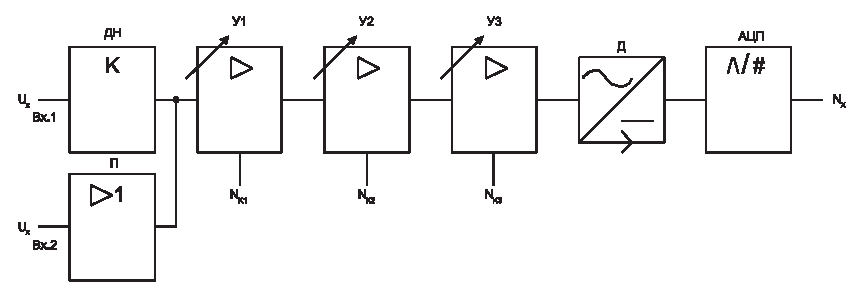
\includegraphics[width=1\textwidth]{./about/func_in}
    \captionsetup{width=170mm,
                margin={200mm,-200mm}
                }%
  \caption{Функциональная схема измерителя напряжения ИН2, необходимая для демонстрации возможностей включения рисунков и корректного переноса подрисуночной подписи} \label{p:func_in2_3}
\end{figure}

приведена функциональная можно найти дополнительные сведения по включению рисунков в документ можно найти дополнительные сведения по включению рисунков в документ рисунков в документ можно найти дополнительные сведения по включению рисунков в документрисунков в документ можно найти дополнительные сведения по включению рисунков в документрисунков в документ можно найти дополнительные сведения по включению рисунков в документрисунков в документ можно найти дополнительные сведения по включению рисунков в документрисунков в документ можно найти дополнительные сведения по включению рисунков в документрисунков в документ можно найти дополнительные сведения по включению рисунков в документрисунков в документ можно найти дополнительные сведения по включению рисунков в документрисунков в документ можно найти дополнительные сведения по включению рисунков в документрисунков в документ можно найти 

%\pagebreak
}%



\FormatSizeA{3}{%

На рисунке~\ref{p:func_in2_1} приведена функциональная можно найти дополнительные сведения по включению рисунков в документ можно найти дополнительные сведения по включению рисунков в документ
схема измерителя напряжения ИН2. В книге \cite{gussens} можно найти дополнительные сведения по включению рисунков в документ.

\begin{figure}[H]
  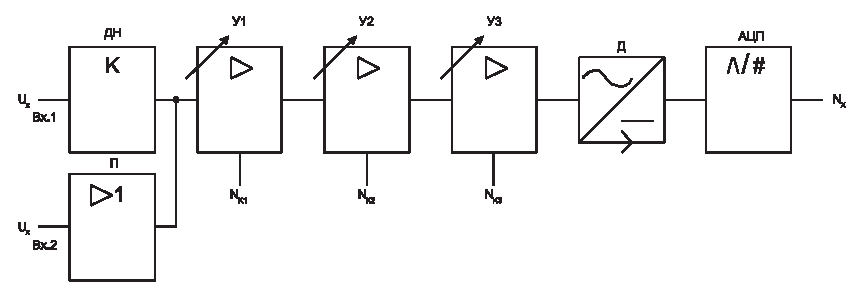
\includegraphics[width=1\textwidth]{./about/func_in}
  \captionsetup{%width=170mm,
                margin={20mm,-200mm}
                }%
  \caption{Функциональная схема измерителя напряжения ИН2, необходимая для демонстрации возможностей включения рисунков и корректного переноса подрисуночной подписи} \label{p:func_in2_4}
\end{figure}

приведена функциональная можно найти дополнительные сведения по включению рисунков в документ можно найти дополнительные сведения по включению рисунков в документ
схема измерителя напряжения ИН2. приведена функциональная можно найти дополнительные сведения по включению рисунков в документ можно найти дополнительные сведения по включению рисунков в документ
схема измерителя напряжения ИН2. приведена функциональная можно найти дополнительные сведения по включению рисунков в документ можно найти дополнительные сведения по включению рисунков в документ
схема измерителя напряжения ИН2. приведена функциональная можно найти дополнительные сведения по включению рисунков в документ можно найти дополнительные сведения по включению рисунков в документ

%\pagebreak
}%


\FormatSizeA{1}{%

На рисунке~\ref{p:func_in2_1} приведена функциональная можно найти дополнительные сведения по включению рисунков в документ можно найти дополнительные сведения по включению рисунков в документ
схема измерителя напряжения ИН2. В книге \cite{gussens} можно найти дополнительные сведения по включению рисунков в документ.

\begin{figure}[H]
  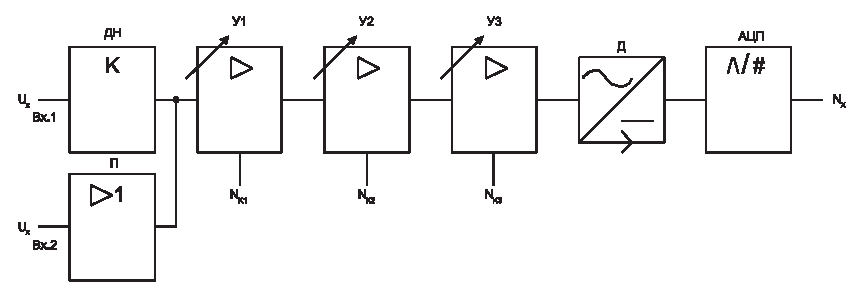
\includegraphics[width=1\textwidth]{./about/func_in}
  \captionsetup{%width=170mm,
                margin={200mm,-400mm}
                }%
  \caption{Функциональная схема измерителя напряжения ИН2, необходимая для демонстрации возможностей включения рисунков и корректного переноса подрисуночной подписи} \label{p:func_in2_4}
\end{figure}

приведена функциональная можно найти дополнительные сведения по включению рисунков в документ можно найти дополнительные сведения по включению рисунков в документ
схема измерителя напряжения ИН2. приведена функциональная можно найти дополнительные сведения по включению рисунков в документ можно найти дополнительные сведения по включению рисунков в документ
схема измерителя напряжения ИН2. приведена функциональная можно найти дополнительные сведения по включению рисунков в документ можно найти дополнительные сведения по включению рисунков в документ
схема измерителя напряжения ИН2. приведена функциональная можно найти дополнительные сведения по включению рисунков в документ можно найти дополнительные сведения по включению рисунков в документ
схема измерителя напряжения ИН2. приведена функциональная можно найти дополнительные сведения по включению рисунков в документ можно найти дополнительные сведения по включению рисунков в документ
схема измерителя напряжения ИН2. приведена функциональная можно найти дополнительные сведения по включению рисунков в документ можно найти дополнительные сведения по включению рисунков в документ
схема измерителя напряжения ИН2. приведена функциональная можно найти дополнительные сведения по включению рисунков в документ можно найти дополнительные сведения по включению рисунков в документ
схема измерителя напряжения ИН2. приведена функциональная можно найти дополнительные сведения по включению рисунков в документ можно найти дополнительные сведения по включению рисунков в документ

%\pagebreak
}%


\FormatSizeA{3}{%

На рисунке~\ref{p:func_in2_1} приведена функциональная можно найти дополнительные сведения по включению рисунков в документ можно найти дополнительные сведения по включению рисунков в документ
схема измерителя напряжения ИН2. В книге \cite{gussens} можно найти дополнительные сведения по включению рисунков в документ.

\begin{figure}[H]
  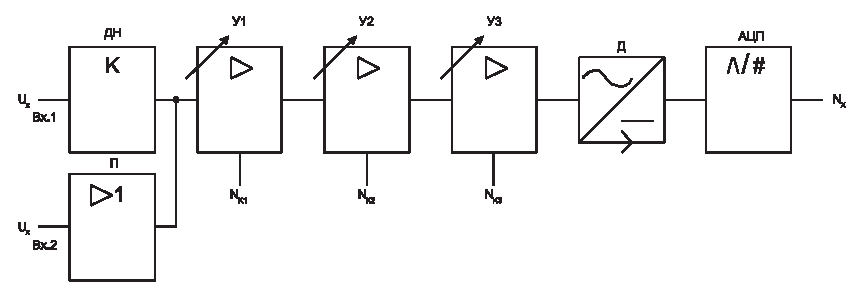
\includegraphics[width=1\textwidth]{./about/func_in}
  \captionsetup{%width=170mm,
                margin={15mm,-200mm}
                }%
  \caption{Функциональная схема измерителя напряжения ИН2, необходимая для демонстрации возможностей включения рисунков и корректного переноса подрисуночной подписи} \label{p:func_in2_4}
\end{figure}

приведена функциональная можно найти дополнительные сведения по включению рисунков в документ можно найти дополнительные сведения по включению рисунков в документ
схема измерителя напряжения ИН2. приведена функциональная можно найти дополнительные сведения по включению рисунков в документ можно найти дополнительные сведения по включению рисунков в документ
схема измерителя напряжения ИН2. приведена функциональная можно найти дополнительные сведения по включению рисунков в документ можно найти дополнительные сведения по включению рисунков в документ
схема измерителя напряжения ИН2. приведена функциональная можно найти дополнительные сведения по включению рисунков в документ можно найти дополнительные сведения по включению рисунков в документ

%\pagebreak
}%




\FormatSizeA{43}{%

На рисунке~\ref{p:func_in2_40} приведена функциональная можно найти дополнительные сведения по включению рисунков в документ можно найти дополнительные сведения по включению рисунков в документ
схема измерителя напряжения ИН2. В книге \cite{gussens} можно найти дополнительные сведения по включению рисунков в документ.


\begin{figure}[H]\center
  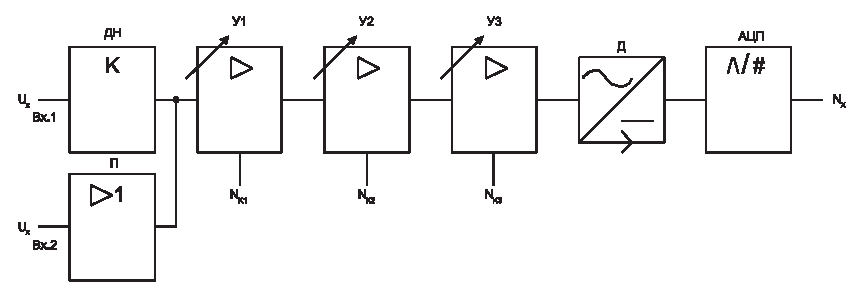
\includegraphics[width=0.7\textwidth]{./about/func_in}
  \captionsetup{%width=170mm,
                margin={15mm,-200mm}
                }%
  \caption{Функциональная схема измерителя напряжения ИН2, необходимая для демонстрации возможностей включения рисунков и корректного переноса подрисуночной подписи} \label{p:func_in2_40}
\end{figure}

приведена функциональная можно найти дополнительные сведения по включению рисунков в документ можно найти дополнительные сведения по включению рисунков в документ
схема измерителя напряжения ИН2. приведена функциональная можно найти дополнительные сведения по включению рисунков в документ можно найти дополнительные сведения по включению рисунков в документ
схема измерителя напряжения ИН2. приведена функциональная можно найти дополнительные сведения по включению рисунков в документ можно найти дополнительные сведения по включению рисунков в документ
схема измерителя напряжения ИН2. приведена функциональная можно найти дополнительные сведения по включению рисунков в документ можно найти дополнительные сведения по включению рисунков в документ

%\pagebreak
}%